\section{Problema 3: Guardando el tesoro}

\subsection{Introducción}

En medio del viaje, nuestros arqueólogos encuentran una sala llena de tesoros, cada uno con un peso y valor determinados, que desean llevar a su casa utilizando las mochilas con las que disponen. Deberán distribuir estos objetos de manera lo suficientemente eficiente como para maximizar el valor total entre todas las mochilas sabiendo que cada una de estas tiene un tope de peso que pueden llevar.

Dicho formalmente, si tenemos un conjunto de $n$ objetos $O = \{(p_i,v_i) \quad | \quad 1 \leq i \leq n\}$ con peso $p_i$ y valor $v_i$ y $m$ mochilas con capacidad $K_j$, queremos seleccionar objetos $o_i$ para cada mochila $M_j$ de manera tal de maximizar $\sum_{j = 0}^m\sum_{o_i \in M_j} v_i$ (es decir, la suma total del valor de cada mochila) sin exceder su capacidad de peso (Osea, $(\sum_{o_i \in M_j} p_i) \leq K_j$).

Este tipo de problema es conocido como Multiple Knapsack.

\subsection{Solución}

Antes de presentar la solución se aclara que, a diferencia de como se presenta en el enunciado, se tienen en cuenta a todos los tesoros como si fueran distintos. Es decir, por ejemplo, si hay 4 unidades de un mismo tesoro, se tienen en cuenta a cada uno como tesoros distintos de igual peso y valor.

Para solucionar el problema, se utilizó programación dinámica de la siguiente manera:

\begin{itemize}
\item Se empieza suponiendo que todas las mochilas tienen capacidad 0. Se van haciendo pruebas sobre mochilas de tamaño creciente hasta haber probado todas las combinaciones de tamaños posibles.
\item Estas pruebas consisten en ver, dada una combinación de capacidades máximas, cuál es la combinación de objetos que genera el máximo valor sin superar la cota de ninguna mochila.
\item Para ver eso, se van probando para cada $i$ posible cuál es el resultado óptimo usando los primeros $i$ objetos. Si el objeto $i$ entra en la mochila $j$, se consulta un valor previamente calculado, el cual es el resultante de hacer este mismo procedimiento con la misma configuración de mochilas, con la diferencia de que a la mochila $j$ se le resta el peso del objeto $i$. Si ese valor sumado al valor del objeto $i$ supera al que venía siendo el candidato a valor máximo, será reemplazado por este mismo.
\end{itemize}

Sobre el último ítem: lo que se hace cuando se consulta el resultado anteriormente calculado es tener en cuenta que hay un invariante en el algoritmo: todos los resultados anteriores (para pesos de mochila menores o usando menos objetos con el peso actual) son el valor óptimo. Entonces, si se pregunta por una combinación en la cual el peso de una de las mochilas es menor, se tiene la seguridad de que eso ya fue calculado y es el mejor valor. Si el objeto $i$ con peso $p_i$ entra en la mochila $j$, se trata de encontrar cuál es la mejor combinación con el peso restante de la mochila $j$, dejando a las otras mochilas intactas y sin tener en cuenta al objeto $i$, usando los $i-1$ anteriores, para luego sumar $p_i$ a la mochila $j$ y $v_i$ al valor total. Otra opción sería no poner el objeto $i$ en ninguna mochila, y por lo tanto el resultado será el mismo que usar $i-1$ objetos con la combinación de pesos actual (que ya tenemos calculado).

Teniendo los resultados para cada posible elección (poner el objeto en una de las mochilas o no ponerlo), seleccionamos como valor óptimo el máximo de los valores. Esta decisión la guardamos en un array multidimensional que nos dice para cada combinación de pesos y para cada objeto en qué mochila lo pusimos (o $-1$ si no lo usamos). Además en todo momento mantenemos un $valorMaximo$ que nos indica con qué combinación de pesos obtuvimos el mejor valor visto.

Al finalizar la corrida sobre todas las combinaciones posibles sabemos la combinación que nos provee el valor máximo, y el valor de este. Para reconstruir la serie de objetos usados empezamos desde el último objeto de la combinación máxima y vemos a dónde lo pusimos. Si no lo colocamos en ningún lugar seguimos con el objeto anterior. Si lo colocamos en la mochila $j$, lo agregamos a la lista de objetos usados y pasamos a considerar la combinación de pesos resultante de restarle el peso del objeto a la mochila $j$ y continuamos con el objeto anterior. Repetimos el proceso recorriendo todos los objetos, y al finalizar tenemos la lista de objetos que queríamos.

Para simplificar el algoritmo consideraremos $valorMaximo = -1$ para representar los casos donde no existe una combinación de los objetos disponibles en las mochilas tal que complete el peso requerido en cada una.

A continuación se presenta el pseudo-código asociado al algoritmo que resuelve el problema:

\begin{lstlisting}
input: mochilas : vector<int>,  objetos : vector<int>

$m \leftarrow$ cantidad de mochilas
mejorValor $\leftarrow$ crear un vector de $m+1$ dimensiones
mochilaUsada $\leftarrow$ crear un vector de $m+1$ dimensiones
int mejorValorGlobal
mejorCombinacion $\leftarrow$ vector de longitud $m$
para toda combinacion $p$ de pesos de mochilas $w_1 \ldots w_m$ (recorridas en un orden creciente)
	int valorCandidato
	para todo $i$ desde $1$ hasta $n$
		valorAnterior  $\leftarrow$ $mejorValor[w_1][w_2]\ldots[w_m][i-1]$
		mochilaUsada$[w_1][w_2]\ldots[w_m][i]$ $\leftarrow$ -1
		para todo $j$ desde $1$ hasta $m$
			si el objeto $i$ entra en la mochila con peso $w_j$
				valCandidato $\leftarrow$ $mejorValor[w_1]\ldots[w_{j-1}][w_j - p_i][w_{j+1}]\ldots[w_m][i-1]$
			sino
				valorCandidato $\leftarrow$ $-1$
			si valorAnterior < valorCandidato
				pongo el objeto en la mochila con peso $w_j$ para esta combinacion
				valorAnterior $\leftarrow$ valorCandidato
				mochilaUsada$[w_1][w_2]\ldots[w_m][i]$ $\leftarrow$ $j$
	si valorCandidato $>$ mejorValorGlobal
		mejorValorGlobal $\leftarrow$ valorCandidato
		mejorCombinacion $\leftarrow$ p

// Reconstruimos los objetos usados
vector<int> objetosUsados
combinacionActual $\leftarrow$ mejorCombinacion // $w_1 \ldots w_m$ son los valores de la combinacion
para $i$ desde $n$ hasta $1$:
    $j$ = mochilaUsada$[w_1][w_2]\ldots[w_m][i]$
    si $j \neq -1$:
        agregar $i$ a objetosUsados
        restarle el peso del objeto $i$ a la mochila $j$ en la combinacion actual

// El resultado esta en mejorValorGlobal y en objetosUsados
\end{lstlisting}

Puntualmente, para recorrer todas las combinaciones de pesos comenzamos con todos en cero y vamos aumentando el peso de la última mochila hasta llegar al máximo, luego la devolvemos a 0 y aumentamos en uno el valor de la mochila anterior. Vamos repitiendo el proceso llevando el \textit{carry} de cada mochila a la anterior hasta llegar a la combinación máxima.

De esta manera nos aseguramos de recorrer todas las combinaciones posibles y que para cada combinación vista ya hayamos calculado el valor de todas las menores.

\subsubsection{Correctitud}

Para demostrar que nuestra solución es correcta, debemos probar que se cumple el invariante que enunciamos anteriormente. Esto es, que conozco los resultados óptimos para cada $i$ primeros objetos para cada combinación menor a la actual. Dado que recorremos los pesos en un orden creciente (para cada peso que vemos ya recorrimos los pesos menores), esto es equivalente a probar optimalidad realizando inducción estructural en las combinaciones de pesos parciales de mochilas. Para ello necesitamos definir la relación de orden parcial bien fundada de la siguiente manera:
\\

Dadas $m$ mochilas y dos vectores de pesos $p$ y $p'$ de dimensión $m$

$$p \leq p' \Leftrightarrow p_i \leq p'_i \quad \forall \quad 1 \leq i \leq m$$

Existe un elemento mínimo $0_m$ que es el vector con ceros en todas sus coordenadas y cumple

$$0_m \leq p \quad \forall p$$

Por lo tanto nuestra relación de orden cumple lo pedido.
\\

Dentro de cada paso inductivo haremos otra inducción sobre la cantidad de objetos que consideramos, probando en cada paso que obtuvimos el óptimo para la los $n$ primeros objetos.

Como nuestro algoritmo recorre los pesos 

\vspace{5mm}

{\Large\textbf{Mochilas: Caso base}}

\vspace{5mm}

Para esta instancia consideramos al menor elemento en nuestro orden de vectores: $0_m$.

\vspace{5mm}

{\large\textbf{Objetos: Caso base}}

\vspace{5mm}

Si tenemos el vector $0_m$ y $0$ objetos, el resultado es trivial ya que el valor máximo es $0$ y para cada mochila se introducen $0$ objetos.

\vspace{5mm}

{\large\textbf{Objetos: Paso inductivo}}

\vspace{5mm}

Para este caso, contamos con el vector $0_m$ y los $n > 0$ primeros objetos. Como los pesos de los objetos son estrictamente positivos, no se puede colocar el objeto $n$ en ninguna mochila y el resultado será el de usar $n-1$ objetos, que calculamos como 0 y es efectivamente el óptimo.

\vspace{5mm}

{\Large\textbf{Mochilas: Paso inductivo}}

\vspace{5mm}

Para esta instancia, dado un vector de pesos $p \neq 0_m$ cualquiera, queremos probar que el algoritmo resuelve el problema sabiendo que puede hacerlo para cualquier vector menor o igual a $p$.

\vspace{5mm}

{\large\textbf{Objetos: Caso base}}

\vspace{5mm}

Si tenemos el vector $p$ y $0$ objetos, el resultado vuelve a ser trivial y no se necesita utilizar la hipótesis inductiva ya que existe una mochila con peso $> 0_m$, pero $0$ objetos para llenarla. Por lo tanto no hay solución y representamos el mejor valor con $-1$.

\vspace{5mm}

{\large\textbf{Objetos: Paso inductivo}}

\vspace{5mm}

Para esta demostración, resulta importante entender las hipótesis con las que se cuenta:

\begin{itemize}
\item Para el vector $p$, el algoritmo sabe resolver todas las instancias del problema con $n$ objetos.
\item Para cualquier vector $p' < p$, el algoritmo sabe resolver todas las instancias del problema con $k$ objetos (donde $k$ es cualquier natural que podría ser mayor a $n$, aunque eso no se usa en esta demostración)
\end{itemize}

Entonces, dado el vector $p$ y $n + 1$ objetos, hay $m + 1$ opciones que conciernen al objeto $n + 1$-ésimo: o no se lo pone en ninguna mochila, o se lo pone en alguna de las $m$ mochilas. La opción que genere el valor máximo será la que solucione el problema.

Si no se lo incluye en ninguna mochila, se resuelve el problema para los $n$ primeros objetos y por hipótesis inductiva (primer ítem) el algoritmo brinda la mejor solución para esa instancia.

Luego, el algoritmo pregunta mochila por mochila si, dado el peso de la mochila $j$, el objeto entra. En caso afirmativo, el resultado para la mochila $j$ será una suma entre el valor del objeto $n + 1$ y la solución del algoritmo para un vector $p'$ tal que

$$p'_i = p_i \quad \forall \quad i \neq j$$

y sea $o$ el peso del objeto $n + 1$

$$p'_j = p_j - o$$

Esto es correcto pues vale el principio de optimalidad para los resultados intermedios. Si la solución usara un valor menor al calculado para $p'$, sumarle el valor del objeto resultaría en un valor menor al de nuestra solución y por lo tanto no sería optimo. Si en cambio usáramos un valor mayor al calculado para $p'$, este último no sería óptimo y contradiríamos nuestra hipótesis inductiva.

Si no existía una solución para $p'_j$ usando los $n$ primeros objetos, tampoco existirá si queremos poner el objeto $n+1$ en la mochila $j$.

Se puede ver que $p' \leq p$, así que, por hipótesis inductiva (segundo ítem) el algoritmo propuesto puede resolver el problema para el vector $p'$ y los $n$ primeros objetos. Dejando eso en claro, el algoritmo puede proponer un valor máximo para los $m + 1$ casos mencionados al principio. El máximo de todos esos valores será la solución al problema con vector $p$ y $n + 1$ objetos.

De esta manera queda probado que, dados un vector de pesos $p$ y $n$ objetos, el algoritmo da una solución correcta para el problema.

Si mantenemos una variable con el mejor valor visto entre todas las combinaciones calculadas tendremos al final el resultado buscado ya que, como vimos anteriormente, recorrimos todas las combinaciones posibles.

\QEDB

\subsubsection{Complejidad}

A continuación se muestra una versión simplificada del pseudocódigo para hacer énfasis en la cantidad de operaciones que se realizan en el algoritmo.

\begin{lstlisting}
inicializar el vector mejorValor
inicializar el vector mochilaUsada
$[\ldots]$

para toda combinacion $p$ de pesos de mochilas $w_1 \ldots w_m$ (recorridas en un orden crecinte)
	$[\ldots]$
	para todo $i$ desde $1$ hasta $n$
		$[\ldots]$
		para todo $j$ desde $1$ hasta $m$
			[Hacer comparaciones y asignaciones]
$[\ldots]$

para cada objeto de $n$ a $1$
	[Hacer comparaciones y asignaciones]

\end{lstlisting}

Recordemos que $n$ es la cantidad total de objetos y $m$ la cantidad de mochilas. Por cuestiones de consistencia con respecto al enunciado, las llamaremos $\sum C_i$ y $M$ respectivamente, además de que se nota como $K_i$ al peso original de la mochila $i$.
\\

Los dos vectores inicializados tienen $(\prod K_i) \times \sum C_i$ elementos, y por lo tanto la inicialización se realiza en $\mathcal{O}((\prod K_i) \times \sum C_i)$.
\\

Analizamos el loop principal por partes:

\begin{itemize}
\item La primera linea recorre todas las mochilas y hace $K_i$ iteraciones por cada una, con lo cual podemos decir que lo que se encuentra adentro del primer ciclo se ejecuta $\prod K_i$ veces

\item El segundo ciclo que recorre todos los objetos, va desde 1 hasta $n = \sum C_i$

\item El tercer ciclo ejecuta una iteración por mochila, por lo cual hace $M$ iteraciones.

\item Lo que se encuentra dentro del tercer ciclo es el siguiente fragmento de código

\begin{lstlisting}
si el objeto $i$ entra en la mochila con peso $w_j$
				valCandidato $\leftarrow$ $mejorValor[w_1]\ldots[w_{j-1}][w_j - p_i][w_{j+1}]\ldots[w_m][i-1]$
			sino
				valorCandidato $\leftarrow$ $-1$
			si valorAnterior < valorCandidato
				pongo el objeto en la mochila con peso $w_j$ para esta combinacion
				valorAnterior $\leftarrow$ valorCandidato
\end{lstlisting}

Todas son comparaciones y asignaciones en tiempo constante (``poner el objeto en la mochila con peso $w_j$'' es hacer una asignación en un vector) por lo cual esto mismo no influye en el cálculo de complejidad del algoritmo
\end{itemize}

Finalmente, la reconstrucción del resultado se ejecuta en $\mathcal{O}(\sum C_i)$.
\\

Teniendo todos estos factores en cuenta, se puede deducir que el algoritmo realiza $\mathcal{O}((\prod K_i) \times M \times \sum C_i + (\prod K_i) \times M \times \sum C_i + \sum C_i) = \mathcal{O}((\prod K_i) \times M \times \sum C_i)$ operaciones.

A continuación se prueba que la complejidad presentada cumple con la cota de $\mathcal{O}((\sum K_i)^M \times \sum C_i)$ establecida por el enunciado.

Ambas complejidades comparten la expresión $\sum C_i$ por lo cual la demostración consistirá en deducir que $(\prod K_i) \times M \in \mathcal{O}((\sum K_i)^M)$

Para simplificar, notaremos $P = \prod K_i$ y $S = (\sum K_i)^M$

Existe una relación entre $S$ y el Teorema multinomial, el cual establece que dados $n, m \in \mathbb{N}$ y $m$ números $x_1, \ldots , x_m$

$$(x_1 + x_2 + \ldots + x_m)^n = \sum_{k_1 + k_2 + \ldots + k_m = n} \binom{n}{k_1, k_2, \ldots , k_m} \prod_{1 \leq t \leq m} x_t^{k_t}$$

donde $\binom{n}{k_1, k_2, \ldots , k_m} = \frac{n!}{k_1! k_2! \ldots k_m!}$

$S$ es un caso particular de este teorema ya que $n = m$. Si bien esta suma puede parecer complicada, nosotros nos centraremos en uno solo de los términos en el cual $k_1 = k_2 = \ldots = k_m = 1$. Llamaremos a ese término $S_1$.

Se puede ver que esto cumple con la condición de la sumatoria ya que

$$k_1 + k_2 + \ldots + k_m = 1 + 1 + \ldots + 1 = m = n$$

Entonces, reemplazando:

$$S_1 = \binom{m}{k_1, k_2, \ldots , k_m} \prod_{1 \leq t \leq m} x_t^{k_t} = \binom{m}{1, 1, \ldots , 1} \prod_{1 \leq t \leq m} x_t^{1} = m! \prod_{1 \leq t \leq m} x_t $$

Notar que si $x_i \geq 0 \quad \forall \quad i$ entonces $S \geq S_1$

Si cambiamos los nombres de las variables del teorema con los nombres de las variables de este problema queda

$$M! \prod K_i = M! \times P \geq M \times P$$

Como $S \geq S_1 \geq M \times P$, queda demostrado que $M \times P = M \times \prod K_i \in \mathcal{O}((\sum K_i)^M)$ y entonces la complejidad propuesta cumple con la cota establecida por el ejercicio.\QEDB

\subsection{Análisis Experimental}

A continuación se presentan una serie de experimentos que ponen a prueba el algoritmo propuesto en esta sección y ayudan a mostrar que la complejidad temporal propuesta anteriormente es correcta.
Dado que la cantidad de operaciones que realiza el algoritmo depende de más de una variable, se separa el análisis en varias secciones en las cuales varía una sola de las variables y el resto se dejan fijas.

Para cada una de las mediciones se realizaron 10 iteraciones de un mismo caso y se registró el tiempo mínimo que tardó en ejecutarse.

\subsubsection{Variando $\sum C_i$}

Dejando fijas las capacidades máximas de cada mochila, se obtuvieron los siguientes resultados de tiempo de ejecución en función de $\sum C_i$ para una, dos y tres mochilas:

\begin{figure}[H]
		\centering
		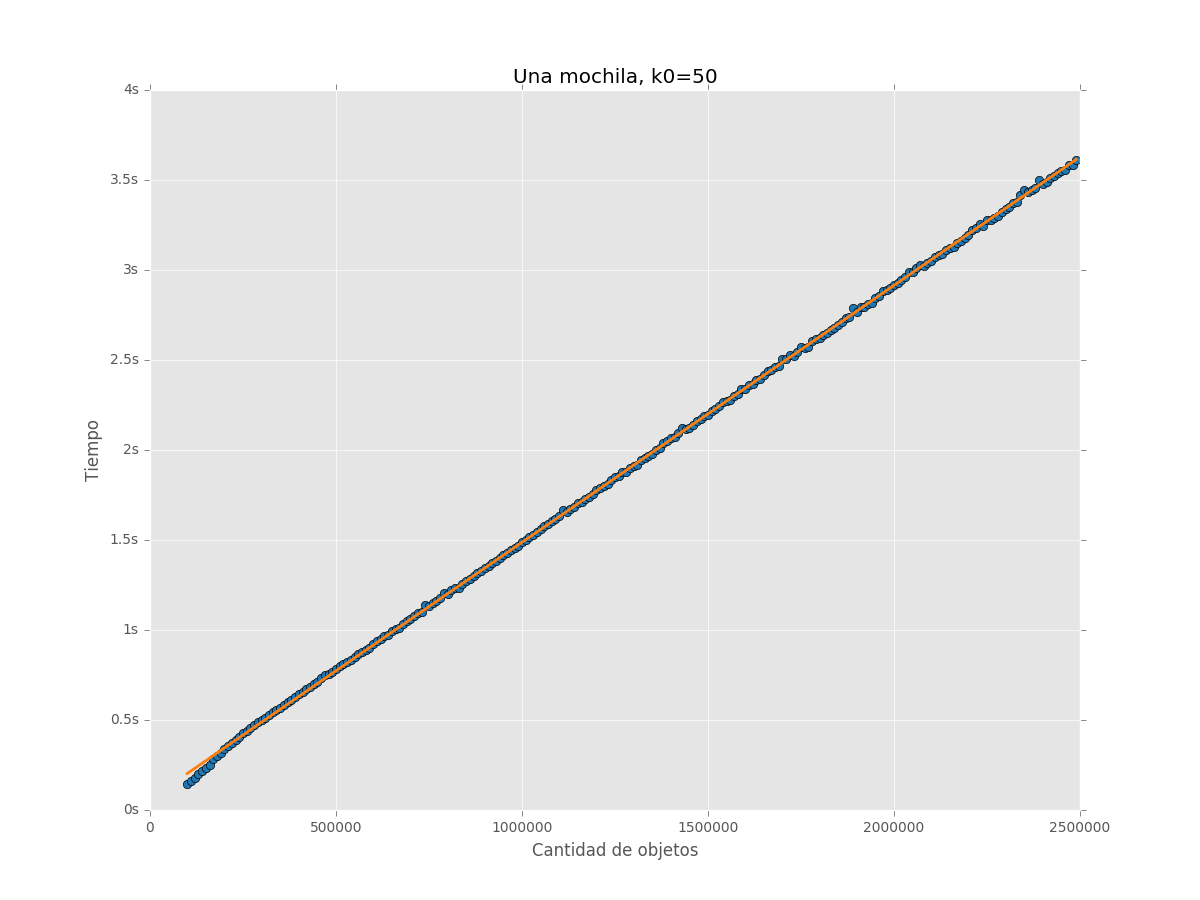
\includegraphics[width=\textwidth]{ej3-c1}
		\caption{Tiempo de ejecución del algoritmo en función de $\sum C_i$ para una mochila}
		\label{fig:ej3-c1-fig}
	\end{figure}

\begin{figure}[H]
		\centering
		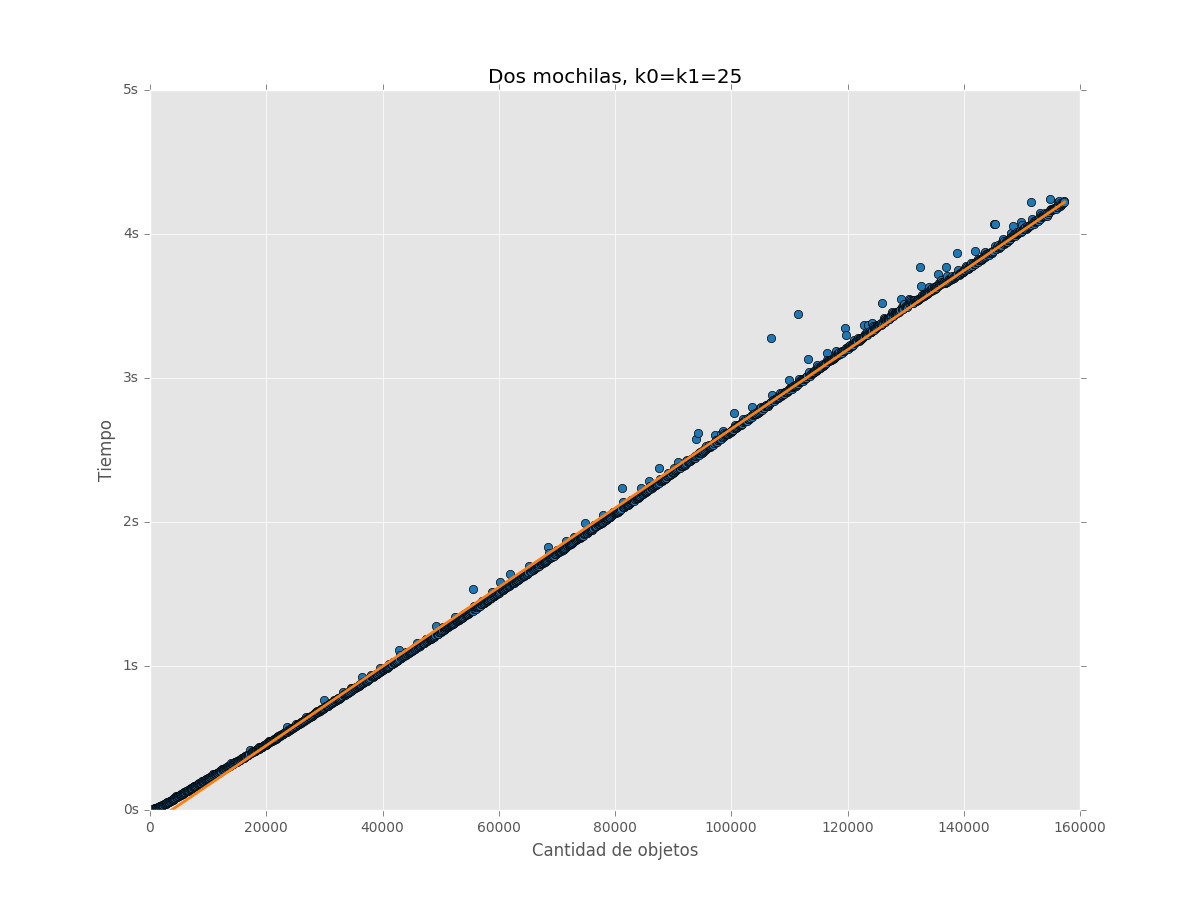
\includegraphics[width=\textwidth]{ej3-c2}
		\caption{Tiempo de ejecución del algoritmo en función de $\sum C_i$ para dos mochilas}
		\label{fig:ej3-c2-fig}
	\end{figure}

\begin{figure}[H]
		\centering
		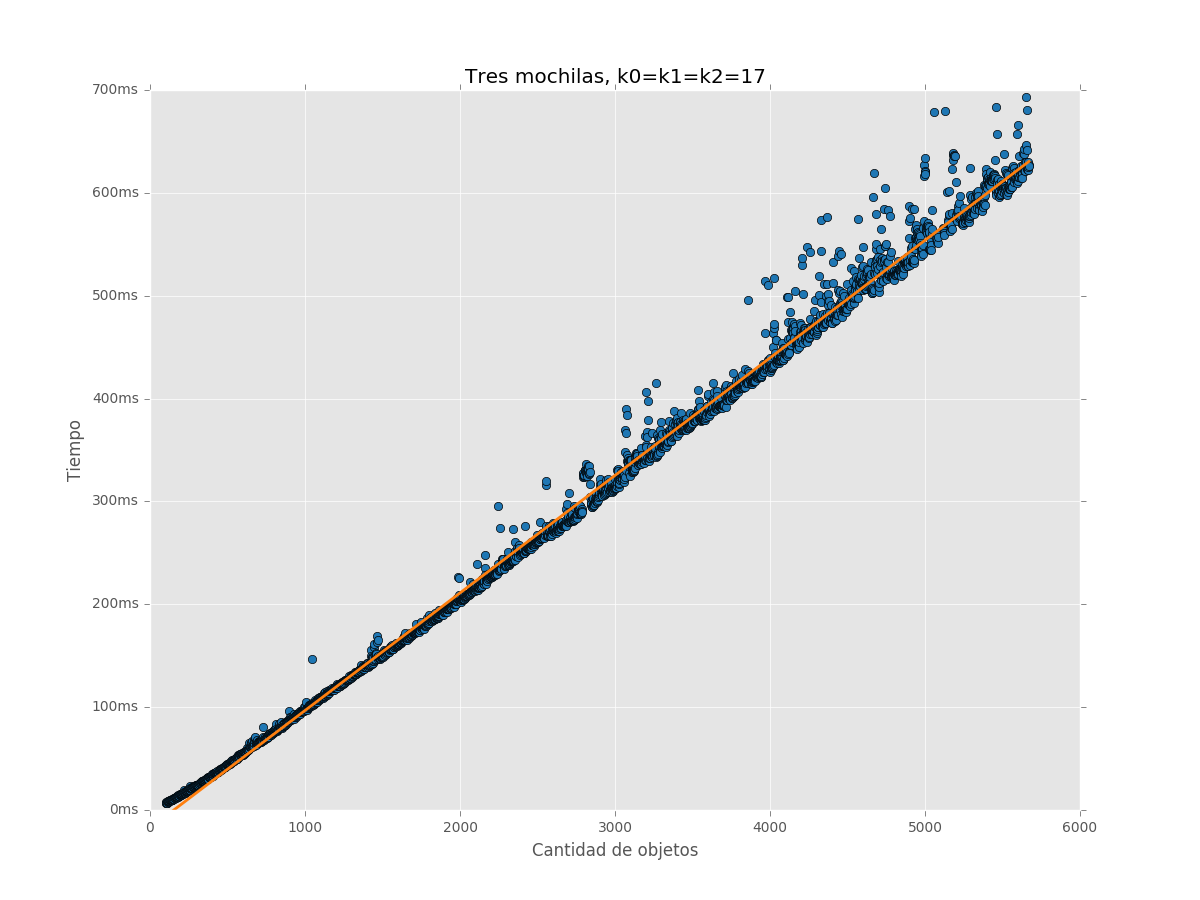
\includegraphics[width=\textwidth]{ej3-c3}
		\caption{Tiempo de ejecución del algoritmo en función de $\sum C_i$ para tres mochilas}
		\label{fig:ej3-c3-fig}
	\end{figure}

Como puede verse en las figuras \ref{fig:ej3-c1-fig}, \ref{fig:ej3-c2-fig} y \ref{fig:ej3-c3-fig}, el algoritmo presenta un comportamiento lineal con respecto a la cantidad de objetos, lo cual es entendible ya que si dejásemos fijos los demás parámetros, la complejidad temporal sería $\mathcal{O}(\sum C_i)$. %Por ahí chamuyé re mal acá. No se que más poner D:

\subsubsection{Variando $\prod K_i$}

Dejando fija la cantidad de objetos, se obtuvieron los siguientes resultados de tiempo de ejecución en función de $\prod K_i$ para una, dos y tres mochilas:

\begin{figure}[H]
		\centering
		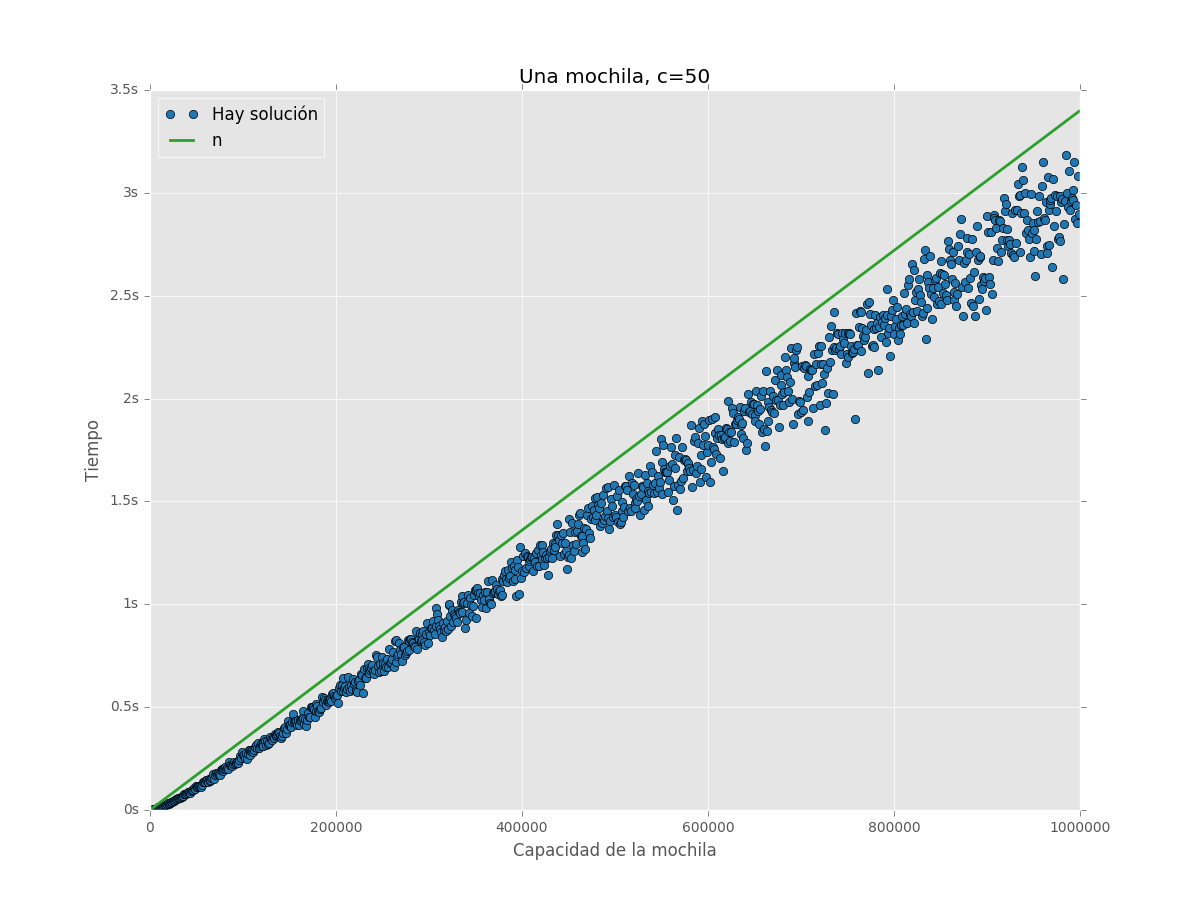
\includegraphics[width=\textwidth]{ej3-k1}
		\caption{Tiempo de ejecución del algoritmo en función de $\prod K_i$ para una mochila}
		\label{fig:ej3-k1-fig}
	\end{figure}

\begin{figure}[H]
		\centering
		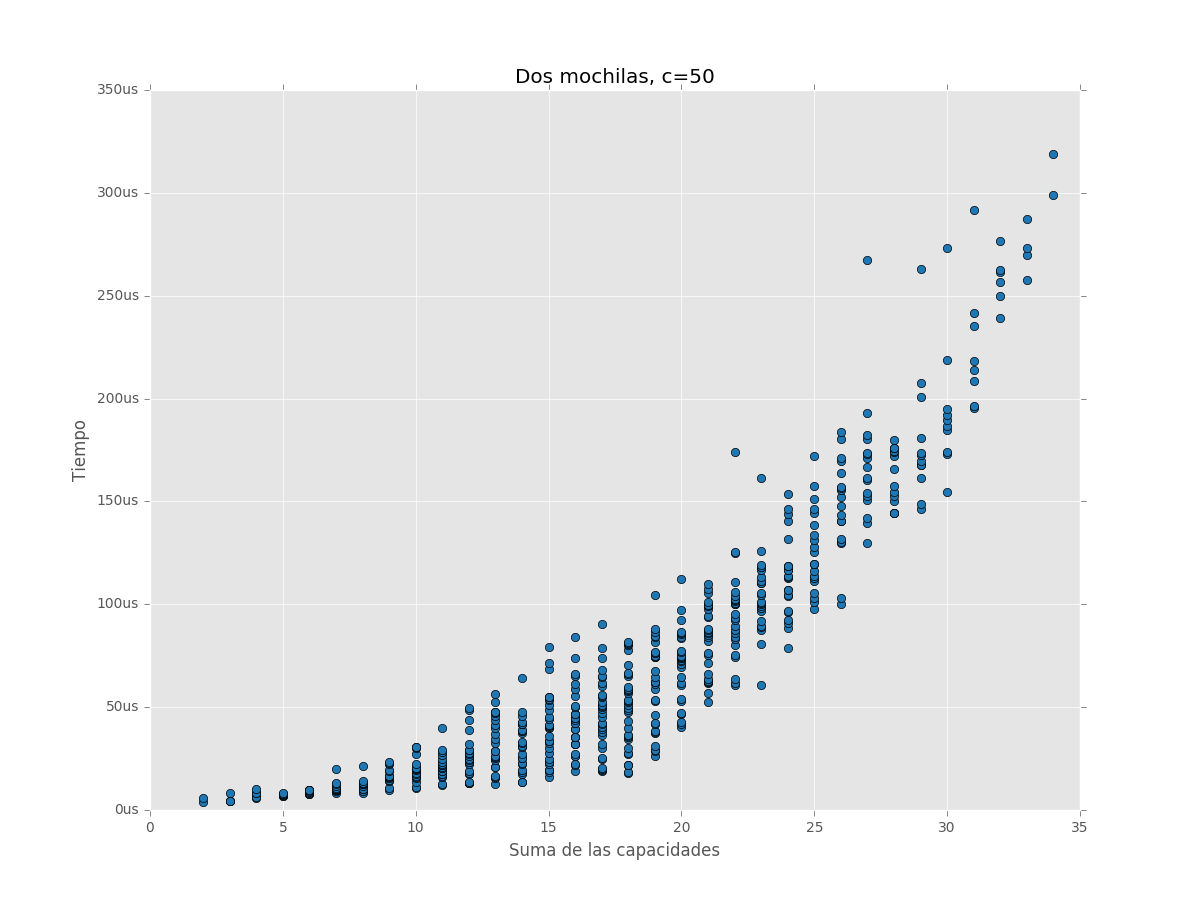
\includegraphics[width=\textwidth]{ej3-k2}
		\caption{Tiempo de ejecución del algoritmo en función de $\prod K_i$ para dos mochilas}
		\label{fig:ej3-k2-fig}
	\end{figure}

\begin{figure}[H]
		\centering
		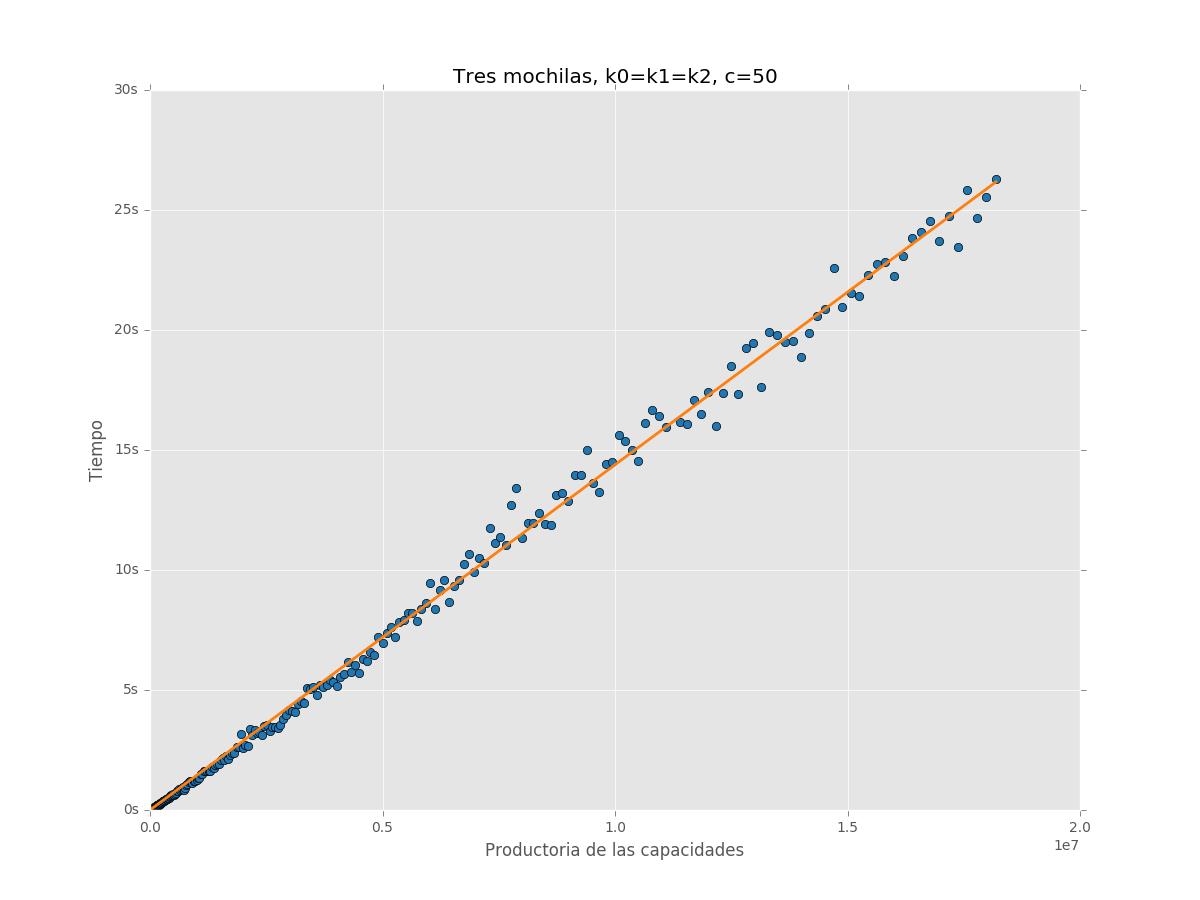
\includegraphics[width=\textwidth]{ej3-k3}
		\caption{Tiempo de ejecución del algoritmo en función de $\prod K_i$ para tres mochilas}
		\label{fig:ej3-k3-fig}
	\end{figure}	

Las figuras \ref{fig:ej3-k1-fig}, \ref{fig:ej3-k2-fig} y \ref{fig:ej3-k3-fig} muestran que si se varía la productoria total de las mochilas, el algoritmo vuelve a presentar un comportamiento lineal, lo cual puede explicarse porque dejando fijas todas las demás variables, el algoritmo tendría una complejidad de $\mathcal{O}(\prod K_i)$. Para generar las mediciones tomamos casos con todas las mochilas iguales y casos con pesos de mochilas aleatorios.

\newpage

Para profundizar más el análisis, se hicieron más experimentos en los que $k_i = k_j$ y se van aumentando de forma lineal todos juntos, de forma tal que $\prod K_i = K_i^M$

\begin{figure}[H]
		\centering
		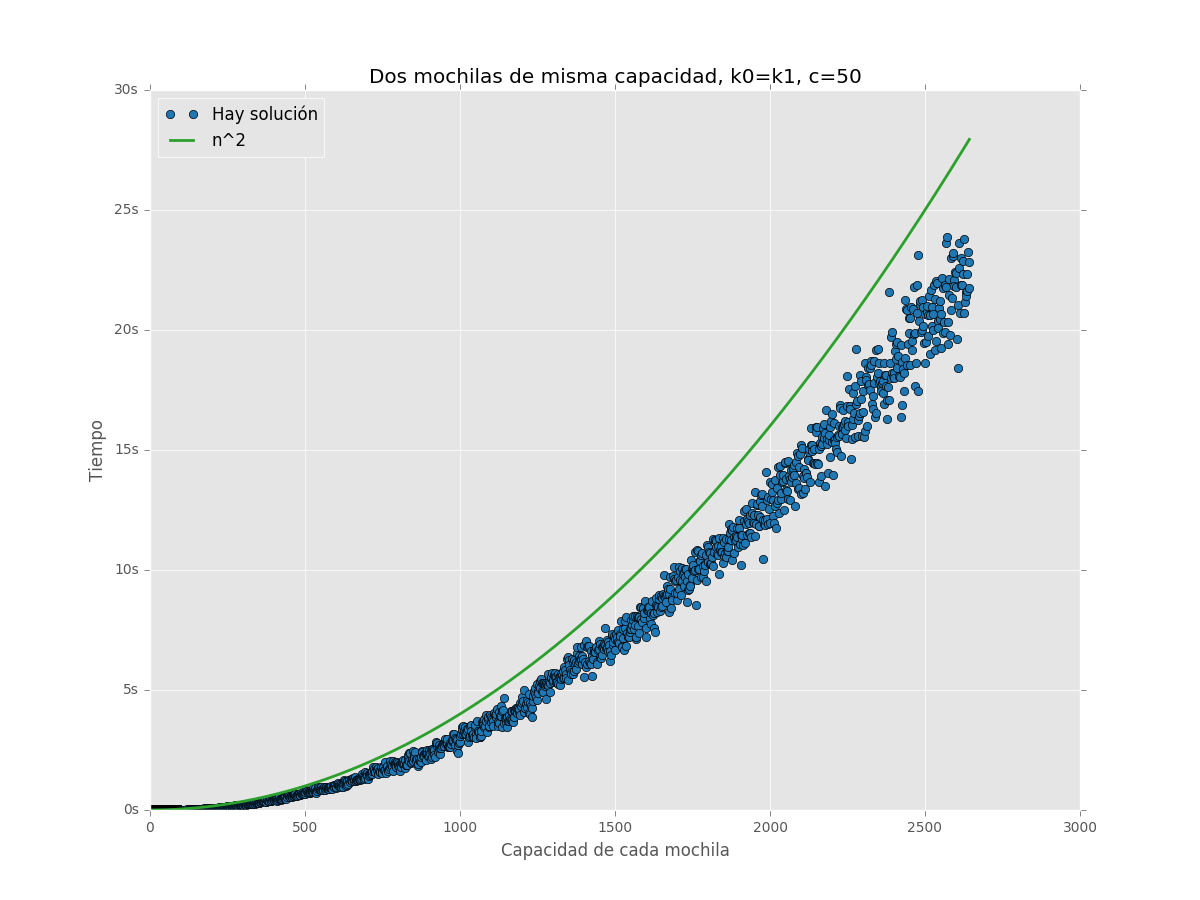
\includegraphics[width=\textwidth]{ej3-k2a}
		\caption{Tiempo de ejecución del algoritmo en función de $K_i$ para dos mochilas. La curva naranja corresponde a un ajuste polinomial de grado 2.}
		\label{fig:ej3-k2a-fig}
	\end{figure}	

\begin{figure}[H]
		\centering
		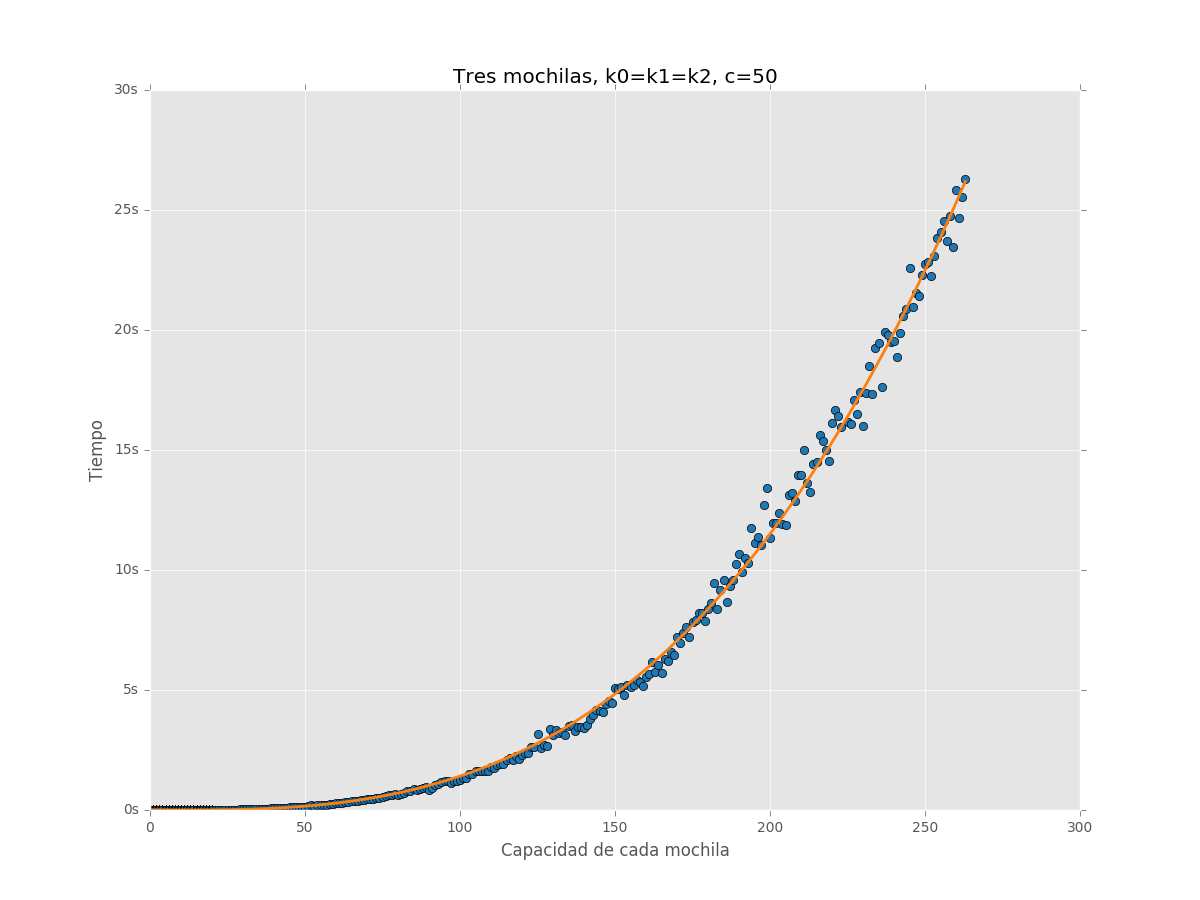
\includegraphics[width=\textwidth]{ej3-k3a}
		\caption{Tiempo de ejecución del algoritmo en función de $K_i$ para tres mochilas. La curva naranja corresponde a un ajuste polinomial de grado 3.}
		\label{fig:ej3-k3a-fig}
	\end{figure}	

En la figura \ref{fig:ej3-k2a-fig} el gráfico presenta un comportamiento cuadrático del algoritmo, y en la figura \ref{fig:ej3-k3a-fig} se ve que el gráfico presenta un comportamiento cúbico. Esto comprueba una vez más las hipótesis de complejidad que fueron presentadas en la sección anterior, ya que evidencia aún más la presencia de la productoria como factor determinante en el tiempo de ejecución.

\subsubsection{Variando $\prod K_i \times \sum C_i$}

Variando la cantidad de objetos al mismo tiempo que la capacidad de una de las mochilas, se obtuvieron los siguientes resultados de tiempo de ejecución en función de $\prod K_i \times \sum C_i$:

\begin{figure}[H]
		\centering
		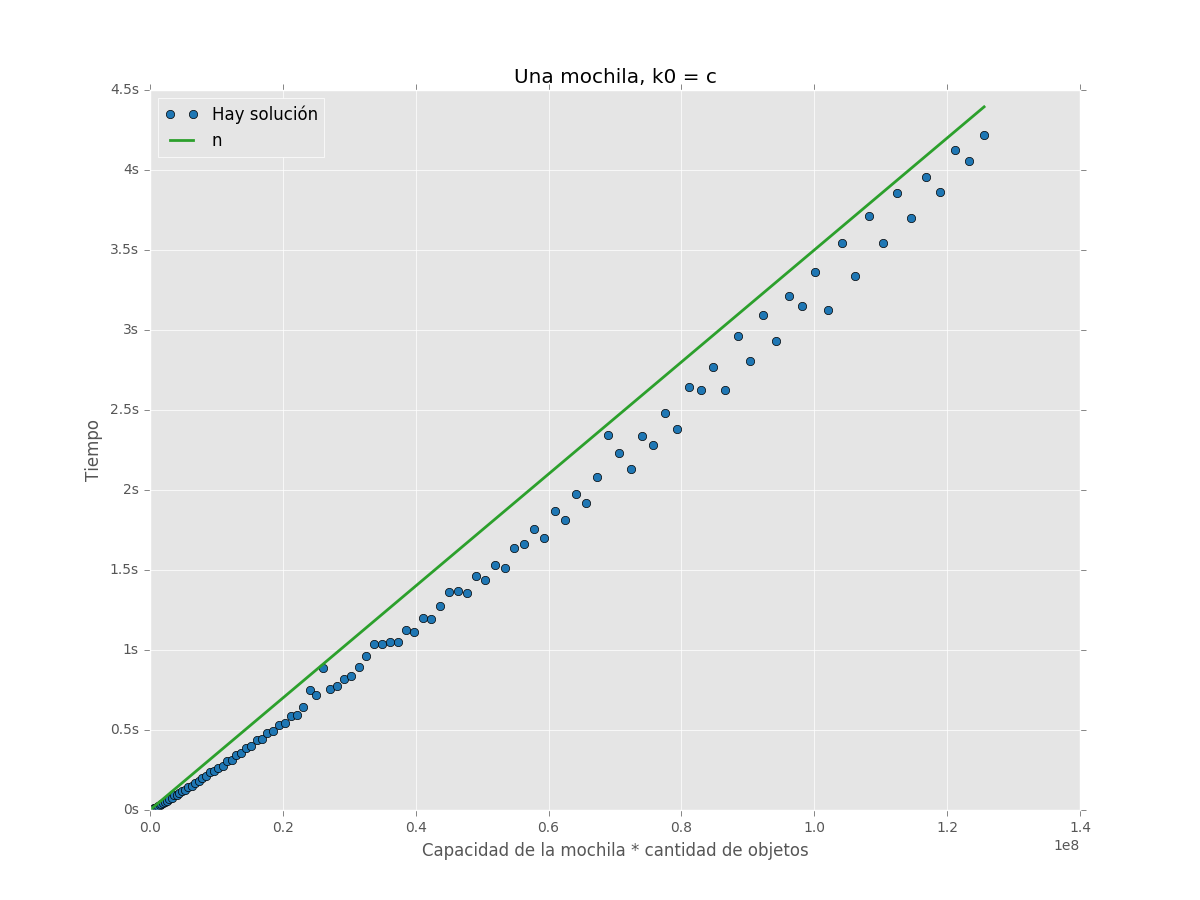
\includegraphics[width=\textwidth]{ej3-mc}
		\caption{Tiempo de ejecución del algoritmo en función de $\prod K_i \times \sum C_i$ para una mochila}
		\label{fig:ej3-mc-fig}
	\end{figure}

Observamos en la figura \ref{fig:ej3-k2a-fig} que efectivamente la complejidad es lineal en función del producto propuesto.

